\begin{frame}{Six-circle diffractometer}

    \begin{columns}
    
        \column[T]{0.5\textwidth}
        \begin{itemize}
            \item $\beta_{in}$ is the incidence angle
            \item $\beta_{out}$ the outgoing angle
            \item $\gamma$ is the out-of-plane detector angle
            \item $\delta$ is the in-plane detector angle
            \item $\omega$ is the sample rotation around the axis perpendicular to the surface or sample azimuth.
        \end{itemize}
        
        In the z-axis mode, $h$ and $k$ are  the in-plane diffraction indices and $l$ is the out-of-plane diffraction index (often perpendicular to the surface). 
        
        $\vec{Q}$ is  the  momentum  transfer: 
        
        \begin{gather}
            \vec{Q} = \Vec{K_f} - \Vec{K_i} \\
            \vec{Q}_{par} = \vec{Q_x} + \vec{Q_y} \\
            \vec{Q_{perp}} = \vec{Q_z}
        \end{gather}
    
        \column[T]{0.5\textwidth}
        \centering
        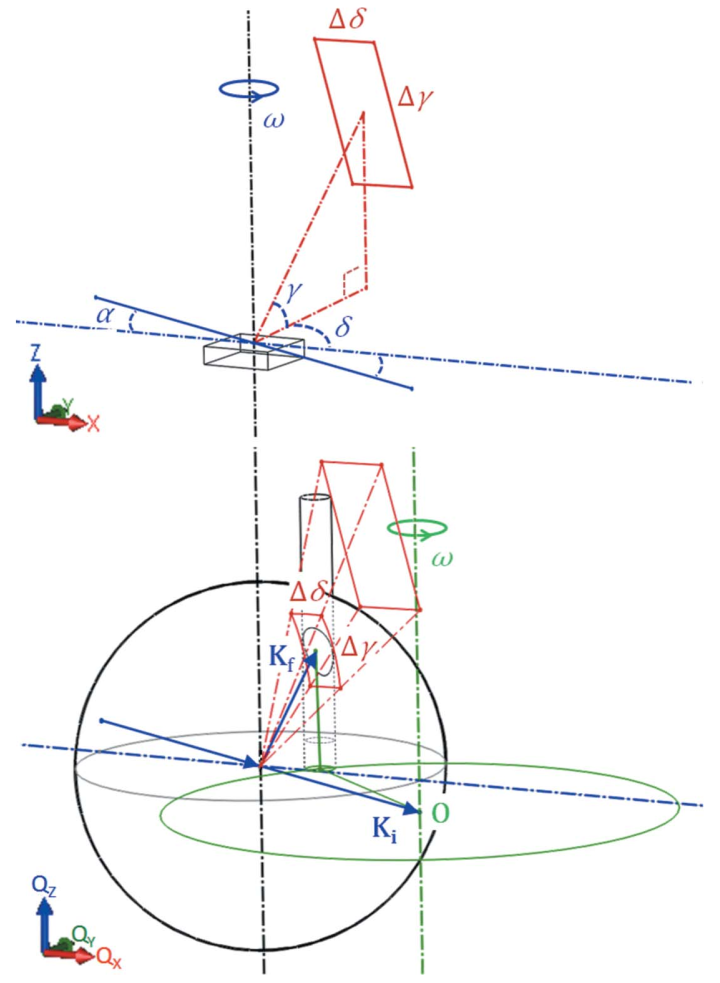
\includegraphics[width=0.8\textwidth]{Figures/sxrd_data/diffracto.png}
    
    \end{columns}

\end{frame}


\begin{frame}{Reciprocal space sampling}

    The integrated intensity of an ideal rocking ($\omega$) scan (i.e. intensity recorded while continuously rotating the sample around its surface normal) is:
    
    \begin{equation}
        I_\omega = \frac{\Phi_0}{\omega_0} \frac{A}{A_u} \int \int \int r_e^2 |F_{hkl}|^2 P u(Q) d\gamma d\delta d\omega
    \end{equation}
    
    \begin{itemize}
        \item $\Phi_0$ incident flux
        \item $\omega_0$ rotation speed
        \item $A$ active surface area
        \item $A_u$ area of the surface unit cell
        \item $|F_{hkl}$ structure factor of the reflection
        \item $P$ polarization factor
        \item and $u(Q)$ line shape function \footnotemark
    \end{itemize}
    
    Omega scans are discrete, with $T_\omega$ the acquisition time and $N_\omega$ points.
    
    \footnotetext{Drnec, J., Zhou, T., Pintea, S., Onderwaater, W., Vlieg, E. (2014). Integration techniques for surface X-ray diffraction data obtained with a two-dimensional detector. Journal of Applied Crystallography, 47, 365–377}

\end{frame}


\begin{frame}{Integrated intensity: rocking scan}

    As the Lorentz factor (L) and polarization factor (P) change with diffraction angle, corrections are necessary to obtain a correct profile, particularly for broad profiles.
    $I_\omega$ can be rewritten with the following correction factors \footnotemark:
    
    \begin{equation}
        I_\omega = \Phi_0 T_\omega \frac{A}{A_u^2} r_e^2 \lambda^2 |F_{hkl}|^2 P C_{area} C_{beam} C_{det} \frac{\Delta\gamma \cos \gamma}{\cos \alpha \sin \delta \cos \gamma}
    \end{equation}
    
    \begin{itemize}
        \item $C_{area}$ area correction factor, proportional to the illuminated surface area, defined by the size of the beam parallel to the surface and by the opening of the slits
        \item $C_{beam}$ compensates for the incoming beam intensity distribution profile
        \item $C_{det}$ present if the in-plane acceptance of the detector is not sufficiently large enough to cover the whole peak
        \item $\frac{1}{\cos \alpha \sin \delta \cos \gamma}$ is the Lorentz factor for the $\omega$ scan
        \item $\cos \gamma$ is the rod interception factor, integration correction dependent on the geometry of the rod–detector interception, assuming that $|F_{hkl}|$ is invariant along $l$ within the considered integration volume
    \end{itemize}
    
    \footnotetext{Vlieg, E. (1997).J. Appl. Cryst.30, 532–543}

\end{frame}

\begin{frame}{Integrated intensity: stationary measurement}

    In the case of a stationary scan, a single data acquisition of duration $T_s$ is carried out at a specific point in the reciprocal space.
    If we consider the in-plane detector acceptance to be larger than the cross section of the rod and $|F_{hkl}|$ to be invariant along $l$ within the intersected area, we have:
    
    \begin{equation}
        I_\omega = \Phi_0 T_\omega \frac{A}{A_u^2} r_e^2 \lambda^2 |F_{hkl}|^2 P C_{area} C_{beam} C_{det} \frac{1}{\sin \gamma}
    \end{equation}
    
    where $\frac{1}{\sin \gamma }$ is the Lorentz factor for the stationary measurements\footnotemark.
    
    \footnotetext{Vlieg, E. (1997).J. Appl. Cryst.30, 532–543}
\end{frame}


\begin{frame}{ROD integration}

    \begin{columns}
    
        \column[T]{0.5\textwidth}

        A complete rod intensity profile is measured through a series of rocking scans at different $l$ values. By using two-dimensional detectors, it is possible to replace each rocking scan by one single stationary measurement centered on the rod at the same $l$ value, speeding up data acquisition. However, certain conditions must be fulfilled:

        \begin{itemize}
            \item The in-plane projection of the finite acceptance of the detector expanded by $K_f\Delta\gamma\sin\gamma$ and $K_f\Delta\delta$ should be sufficiently large to fully include the cross section of the rod. This is not always true as $sin \gamma$ vanishes at $\gamma = 0$. Hence, for low $l$ values, one often has to employ a rocking scan or attempt to compensate for the missing intensity either analytically or numerically.
            \item $|F_{hkl}|$ should be approximately constant over the intersected $l$ range $\Delta l$.
        \end{itemize}
    
        \column[T]{0.5\textwidth}
        \centering
        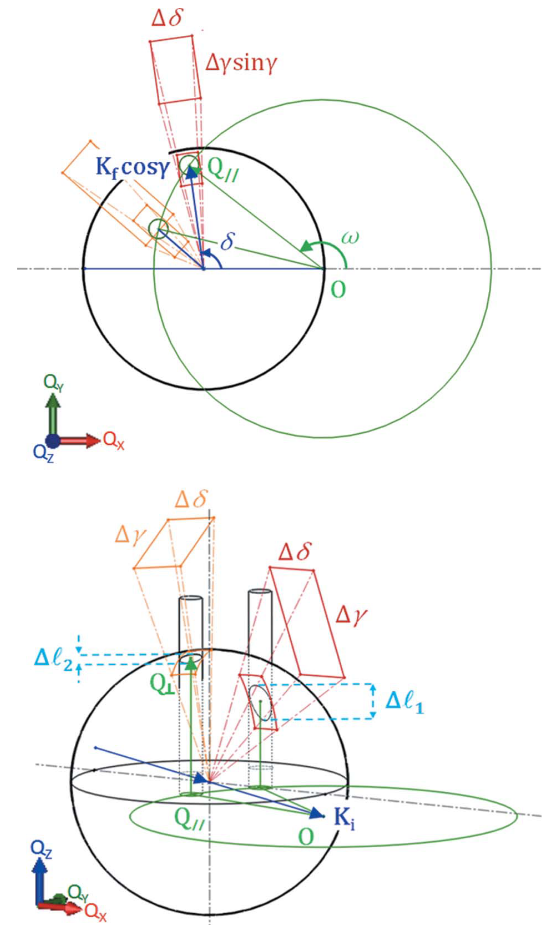
\includegraphics[width=0.7\textwidth]{Figures/sxrd_data/rod_integration.png}
    
    \end{columns}

\end{frame}


\begin{frame}{Background estimation}

    \begin{itemize}
        \item The field of view of the detector should be large enough to fully intersect the rod and accept an area with background intensity.
        \item Over (or under)-estimation of the background may result in significant errors.
        \begin{enumerate}
            \item Calculate the overall integrated intensity inside a region of interest (RoI) covering the intercepted rod
            \item Subtract the background intensity taken elsewhere.
        \end{enumerate}
        \item Signals coming from outside the sample may be found in close vicinity to the peak or even overlapping the peak, making it impossible to isolate the peak from the background with a regularly shaped RoI (e.g.rectangle).
        \item Applying an irregularly shaped RoI (e.g.a polygon) can solve the problem but requires the RoI to be determined for each image as the peak shape evolves during the scan.
        \item An alternative is to use peak shape determination and background subtraction employing a two-dimensional \textbf{peak search algorithm, detailed in Vlieg et al. (2016)}.
    \end{itemize}

    \centering
    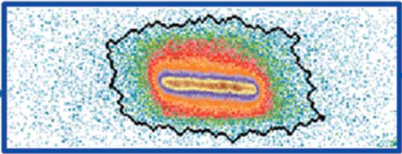
\includegraphics[height=0.25\textheight]{Figures/sxrd_data/SXRD_peak.png}
    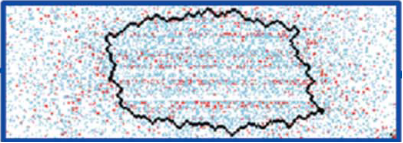
\includegraphics[height=0.25\textheight]{Figures/sxrd_data/SXRD_peak_background.png}
        
\end{frame}


\begin{frame}{Reciprocal space integration}

    The integrated intensity of a given volume in the angular space of the detector is:
    
    \begin{equation}
        I_{int,a} = \Phi_0 T_r \int \int \int \frac{d\sigma}{d\Omega}(\vec{Q})d\gamma d\psi d\phi
    \end{equation}
    
    where $\Phi_0$ is the incident flux, $T_r$ the counting time, $\frac{d\sigma}{d\Omega}(\vec{Q})$ the differential cross section and $d\gamma d\psi d\phi$ is the integration volume.
    
    The Lorentz correction, $L$, accounts for the angular to reciprocal space volume transformation:
    $d\gamma  d\psi d\phi = \frac{\lambda^3}{V_u} L \, dh \, dk \, dl$. In reciprocal space:
    
    \begin{gather}
        I_{int,r} = \Phi_0 T_r \int \int \int \frac{d\sigma}{d\Omega}(\vec{Q})\, dh \, dk \, dl \\
        I_{int,a} = \frac{\lambda^3}{V_u} L I_{int,r}
    \end{gather}
    
    where $V_u$ is the volume of the unit cell. For stationnary scans we have instead:
    
    \begin{equation}
        I_{int,a} = \frac{\lambda^2}{A_u} L I_{int,r}
    \end{equation}
    
    where $A_u$ is the area of the surface unit cell. The Lorentz correction is included when the pixel intensities of two-dimensional images are converted to the three-dimensional reciprocal space intensity map.

\end{frame}

\begin{frame}{Structure factor}

    The range in $l$ direction, $\Delta l$, measured by a detector is not constant and varies with the component of the scattering vector perpendicular to the surface ($\vec{Q_{perp}}$) and the angle $\gamma$ in the angular space of a detector.

    \begin{itemize}
        \item This is taken into account with the $\cos \gamma$ rod interception factor.
        \item If the integration is done directly in reciprocal space, $\Delta l$ can be chosen to be the same for each $l$ value given that the reciprocal space map has enough data points.
    \end{itemize}
    
    Assuming that $\Delta l$ is small enough so that $\frac{d\sigma}{d\Omega}(\vec{Q})$ is constant within $\Delta l$ we can write:

    \begin{align}
        I_{int,r} = \Phi_0 T_r \int \int \int \frac{d\sigma}{d\Omega}(\vec{Q})\, dh \, dk \, dl \\
        = \Phi_0 T_r \Delta l \int \int \frac{d\sigma}{d\Omega}(\vec{Q})\, dh \, dk \\
        = \Phi_0 T_r \frac{A}{A_u} r_e^2 |F_{hkl}|^2 P C_{area} C_{beam} \Delta l 
    \end{align}


    The $C_{det}$ correction is omitted because, it is possible to recover the in-plane shape and intensity distribution of the rod even if the post sample slit width is smaller than the width of the reflection at the camera distance.
        
\end{frame}

\begin{frame}{Rod integration}

    \begin{itemize}
        \item Is it correct to perform interpolations in the hk plane ?
        \item Do you have $\frac{\partial F_{hkl}}{\partial l} = 0$ ? Is it the correct step in l ?
        \item If in reciprocal space, have you well aligned the sample ? Does the peak move ?
        \item Have you correctly subtracted the background ? I.e. did you take care to see if there are alien peaks / background features ?
        \item Did you fit or integrate the CTR ? Recalculated  or integrated intensities ? Peak shape ?
    \end{itemize}

    \begin{figure}
        \centering
        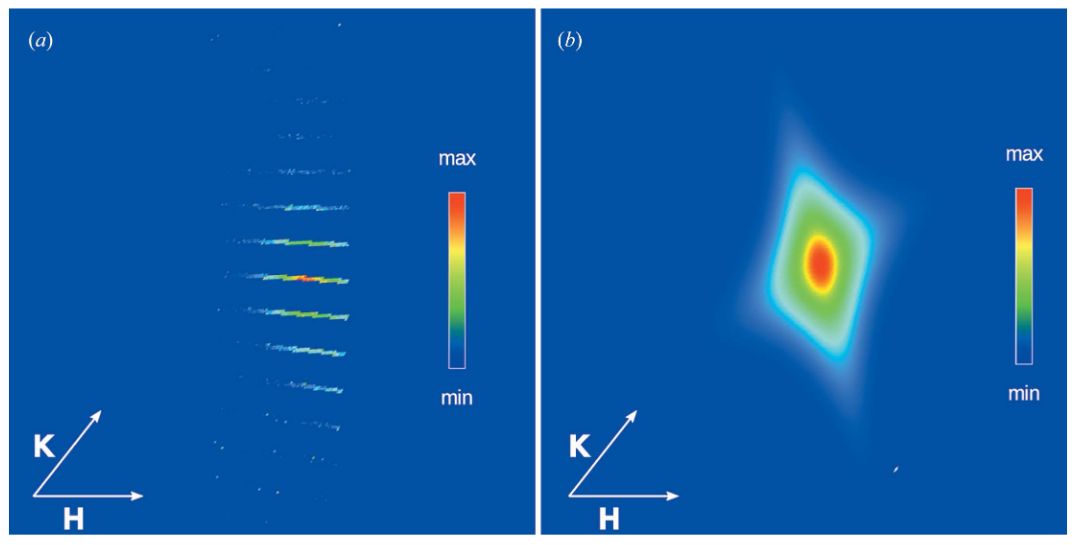
\includegraphics[width=0.6\textwidth]{Figures/sxrd_data/LorentzianFit.png}
        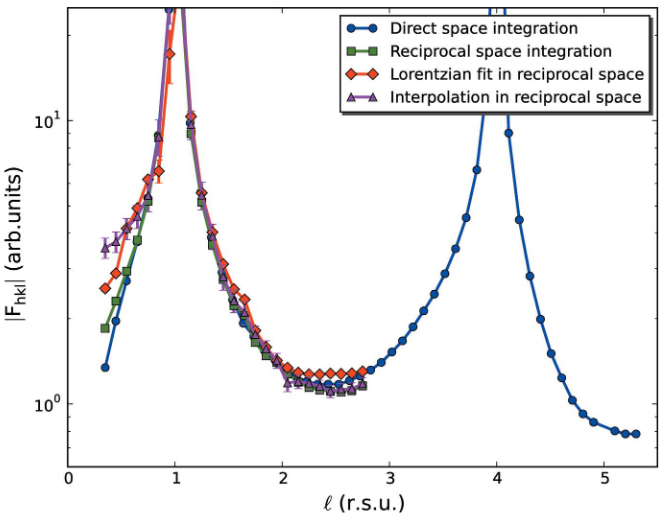
\includegraphics[width=0.38\textwidth]{Figures/sxrd_data/int_dif_sxrd.png}
        \caption{Lorentzian fit (left) and differences in data integration (right).}
        \label{fig:sxrd_data}
    \end{figure}
    
\end{frame}